% Options for packages loaded elsewhere
\PassOptionsToPackage{unicode}{hyperref}
\PassOptionsToPackage{hyphens}{url}
%
\documentclass[
  17pt,
  letterpaper,
  ignorenonframetext,
  aspectratio=169,
  xcolor={dvipsnames}]{beamer}
\usepackage{pgfpages}
\setbeamertemplate{caption}[numbered]
\setbeamertemplate{caption label separator}{: }
\setbeamercolor{caption name}{fg=normal text.fg}
\beamertemplatenavigationsymbolsempty
% Prevent slide breaks in the middle of a paragraph
\widowpenalties 1 10000
\raggedbottom
\setbeamertemplate{part page}{
  \centering
  \begin{beamercolorbox}[sep=16pt,center]{part title}
    \usebeamerfont{part title}\insertpart\par
  \end{beamercolorbox}
}
\setbeamertemplate{section page}{
  \centering
  \begin{beamercolorbox}[sep=12pt,center]{part title}
    \usebeamerfont{section title}\insertsection\par
  \end{beamercolorbox}
}
\setbeamertemplate{subsection page}{
  \centering
  \begin{beamercolorbox}[sep=8pt,center]{part title}
    \usebeamerfont{subsection title}\insertsubsection\par
  \end{beamercolorbox}
}
\AtBeginPart{
  \frame{\partpage}
}
\AtBeginSection{
  \ifbibliography
  \else
    \frame{\sectionpage}
  \fi
}
\AtBeginSubsection{
  \frame{\subsectionpage}
}

\usepackage{amsmath,amssymb}
\usepackage{lmodern}
\usepackage{iftex}
\ifPDFTeX
  \usepackage[T1]{fontenc}
  \usepackage[utf8]{inputenc}
  \usepackage{textcomp} % provide euro and other symbols
\else % if luatex or xetex
  \usepackage{unicode-math}
  \defaultfontfeatures{Scale=MatchLowercase}
  \defaultfontfeatures[\rmfamily]{Ligatures=TeX,Scale=1}
  \setmainfont[BoldFont = SF Pro Text Semibold, Scale =
MatchLowercase]{SF Pro Text Light}
\fi
\usecolortheme{wolverine}
\usefonttheme{serif} % use mainfont rather than sansfont for slide text
\useinnertheme{default}
\useoutertheme{miniframes}
% Use upquote if available, for straight quotes in verbatim environments
\IfFileExists{upquote.sty}{\usepackage{upquote}}{}
\IfFileExists{microtype.sty}{% use microtype if available
  \usepackage[]{microtype}
  \UseMicrotypeSet[protrusion]{basicmath} % disable protrusion for tt fonts
}{}
\makeatletter
\@ifundefined{KOMAClassName}{% if non-KOMA class
  \IfFileExists{parskip.sty}{%
    \usepackage{parskip}
  }{% else
    \setlength{\parindent}{0pt}
    \setlength{\parskip}{6pt plus 2pt minus 1pt}}
}{% if KOMA class
  \KOMAoptions{parskip=half}}
\makeatother
\usepackage{xcolor}
\newif\ifbibliography
\setlength{\emergencystretch}{3em} % prevent overfull lines
\setcounter{secnumdepth}{-\maxdimen} % remove section numbering


\providecommand{\tightlist}{%
  \setlength{\itemsep}{0pt}\setlength{\parskip}{0pt}}\usepackage{longtable,booktabs,array}
\usepackage{calc} % for calculating minipage widths
\usepackage{caption}
% Make caption package work with longtable
\makeatletter
\def\fnum@table{\tablename~\thetable}
\makeatother
\usepackage{graphicx}
\makeatletter
\def\maxwidth{\ifdim\Gin@nat@width>\linewidth\linewidth\else\Gin@nat@width\fi}
\def\maxheight{\ifdim\Gin@nat@height>\textheight\textheight\else\Gin@nat@height\fi}
\makeatother
% Scale images if necessary, so that they will not overflow the page
% margins by default, and it is still possible to overwrite the defaults
% using explicit options in \includegraphics[width, height, ...]{}
\setkeys{Gin}{width=\maxwidth,height=\maxheight,keepaspectratio}
% Set default figure placement to htbp
\makeatletter
\def\fps@figure{htbp}
\makeatother

\captionsetup[figure]{labelformat=empty}
\usepackage{pgfpages}
\setbeamertemplate{itemize item}[circle]
\setbeamertemplate{footline}[frame number]{}
\mode<handout>{\pgfpagesuselayout{6 on 1}[letterpaper, border shrink=8mm]}
\AtBeginSection{%
   \begin{frame}
       \tableofcontents[currentsection]
   \end{frame}
}
\makeatletter
\makeatother
\makeatletter
\makeatother
\makeatletter
\@ifpackageloaded{caption}{}{\usepackage{caption}}
\AtBeginDocument{%
\ifdefined\contentsname
  \renewcommand*\contentsname{Table of contents}
\else
  \newcommand\contentsname{Table of contents}
\fi
\ifdefined\listfigurename
  \renewcommand*\listfigurename{List of Figures}
\else
  \newcommand\listfigurename{List of Figures}
\fi
\ifdefined\listtablename
  \renewcommand*\listtablename{List of Tables}
\else
  \newcommand\listtablename{List of Tables}
\fi
\ifdefined\figurename
  \renewcommand*\figurename{Figure}
\else
  \newcommand\figurename{Figure}
\fi
\ifdefined\tablename
  \renewcommand*\tablename{Table}
\else
  \newcommand\tablename{Table}
\fi
}
\@ifpackageloaded{float}{}{\usepackage{float}}
\floatstyle{ruled}
\@ifundefined{c@chapter}{\newfloat{codelisting}{h}{lop}}{\newfloat{codelisting}{h}{lop}[chapter]}
\floatname{codelisting}{Listing}
\newcommand*\listoflistings{\listof{codelisting}{List of Listings}}
\makeatother
\makeatletter
\@ifpackageloaded{caption}{}{\usepackage{caption}}
\@ifpackageloaded{subcaption}{}{\usepackage{subcaption}}
\makeatother
\makeatletter
\@ifpackageloaded{tcolorbox}{}{\usepackage[many]{tcolorbox}}
\makeatother
\makeatletter
\@ifundefined{shadecolor}{\definecolor{shadecolor}{rgb}{.97, .97, .97}}
\makeatother
\makeatletter
\makeatother
\ifLuaTeX
  \usepackage{selnolig}  % disable illegal ligatures
\fi
\IfFileExists{bookmark.sty}{\usepackage{bookmark}}{\usepackage{hyperref}}
\IfFileExists{xurl.sty}{\usepackage{xurl}}{} % add URL line breaks if available
\urlstyle{same} % disable monospaced font for URLs
\hypersetup{
  pdftitle={Knowledge and Reality, Lecture 18},
  pdfauthor={Brian Weatherson},
  hidelinks,
  pdfcreator={LaTeX via pandoc}}

\title{Knowledge and Reality, Lecture 18}
\author{Brian Weatherson}
\date{11/2/22}

\begin{document}
\frame{\titlepage}
\ifdefined\Shaded\renewenvironment{Shaded}{\begin{tcolorbox}[boxrule=0pt, frame hidden, interior hidden, borderline west={3pt}{0pt}{shadecolor}, sharp corners, enhanced, breakable]}{\end{tcolorbox}}\fi

\hypertarget{a-grand-theory-of-perception}{%
\section{A Grand Theory of
Perception}\label{a-grand-theory-of-perception}}

\begin{frame}{Four Steps}
\protect\hypertarget{four-steps}{}
\begin{enumerate}[<+->]
\tightlist
\item
  Physical world \(\rightarrow\) sensory irritations
\item
  Sensory irritations \(\rightarrow\) experiences
\item
  Experiences \(\rightarrow\) beliefs
\item
  Beliefs \(\rightarrow\) actions
\end{enumerate}
\end{frame}

\begin{frame}{World to Inputs}
\protect\hypertarget{world-to-inputs}{}
We mostly think this is a matter for the scientists to discover.

\begin{itemize}[<+->]
\tightlist
\item
  But note that there are two kinds of philosopher who disagree.
\end{itemize}
\end{frame}

\begin{frame}{World to Inputs}
\protect\hypertarget{world-to-inputs-1}{}
Sceptics think that there may not be an external world.

\begin{itemize}[<+->]
\tightlist
\item
  And if not, the external world can't cause sensory irritations.
\item
  But we're by and large setting them aside.
\item
  For this part of the course, assume there is an external world, and it
  is much like science says it is.
\end{itemize}
\end{frame}

\begin{frame}{World to Input}
\protect\hypertarget{world-to-input}{}
Idealists (in this sense of idealist) deny that the external world is
\emph{physical}.

\begin{itemize}[<+->]
\tightlist
\item
  They think that the world is in some sense fundamentally mental.
\item
  Perhaps the entire world is a construction out of (perhaps merely
  possible) sense-experiences.
\end{itemize}
\end{frame}

\begin{frame}{World to Input}
\protect\hypertarget{world-to-input-1}{}
Idealists (in this sense of idealist) deny that the external world is
\emph{physical}.

\begin{itemize}[<+->]
\tightlist
\item
  Again, set that view to one side, though until recently it was
  \emph{very} popular in Western philosophy.
\end{itemize}
\end{frame}

\begin{frame}{Inputs to Experiences}
\protect\hypertarget{inputs-to-experiences}{}
We don't see firing rates in the optic nerve, or hear vibrations in the
inner ear.

\begin{itemize}[<+->]
\tightlist
\item
  It's only when these things are converted into experiences that we
  have perceptions.
\item
  There are a few reasons to think that we are sensitive to things that
  we don't consciously experience - e.g., blindsight, or very fast
  reactions.
\end{itemize}
\end{frame}

\begin{frame}{Inputs to Experiences}
\protect\hypertarget{inputs-to-experiences-1}{}
We don't see firing rates in the optic nerve, or hear vibrations in the
inner ear.

\begin{itemize}[<+->]
\tightlist
\item
  But we'll mostly pay attention to things where the is a conscious
  experience.
\end{itemize}
\end{frame}

\begin{frame}{Inputs to Experiences}
\protect\hypertarget{inputs-to-experiences-2}{}
I'll sometimes call these things `appearances' or `looks', when talking
about visual experience.

\begin{itemize}[<+->]
\tightlist
\item
  These are all meant to be the same kind of thing.
\item
  As we get further into the book, we'll fuss more about some details
  here.
\end{itemize}
\end{frame}

\begin{frame}{Experiences to Beliefs}
\protect\hypertarget{experiences-to-beliefs}{}
We don't believe everything we see.

\begin{itemize}[<+->]
\tightlist
\item
  Sometimes we ignore it. Actually most of the time I guess that's true;
  I have almost no beliefs about the periphery of my vision most of the
  time.
\item
  Sometimes we overrule it, when we think something must be illusory.
\end{itemize}
\end{frame}

\begin{frame}{Experiences to Beliefs}
\protect\hypertarget{experiences-to-beliefs-1}{}
We don't believe everything we see.

\begin{itemize}[<+->]
\tightlist
\item
  But we're interested in perception because so often we do take things
  to be as they appear.
\end{itemize}
\end{frame}

\begin{frame}{Beliefs to Action}
\protect\hypertarget{beliefs-to-action}{}
And sometimes belief leads to action.

\begin{itemize}[<+->]
\tightlist
\item
  Not always in the way that would be optimal
\item
  Sometimes there is a deer in the headlights effect
\item
  Sometimes someone is committed to an action and does it even when they
  know by perception it would be wrong/pointles.
\item
  But often enough.
\end{itemize}
\end{frame}

\begin{frame}{Four Steps}
\protect\hypertarget{four-steps-1}{}
\begin{enumerate}[<+->]
\tightlist
\item
  Physical world \(\rightarrow\) sensory irritations
\item
  Sensory irritations \(\rightarrow\) experiences
\item
  Experiences \(\rightarrow\) beliefs
\item
  Beliefs \(\rightarrow\) actions
\end{enumerate}
\end{frame}

\begin{frame}{Where Does Philosophy Fit In?}
\protect\hypertarget{where-does-philosophy-fit-in}{}
A simple view:

\begin{itemize}[<+->]
\tightlist
\item
  No role for philosophy at steps 1 and 2; they are just scientific
  question.
\item
  Epistemology has a lot to say about step 3, about how beliefs are
  formed.
\item
  And practical philosophy (ethics, philosophy of action) has a lot to
  say about step 4.
\end{itemize}
\end{frame}

\begin{frame}{Where Does Philosophy Fit In?}
\protect\hypertarget{where-does-philosophy-fit-in-1}{}
Siegel's view:

\begin{itemize}[<+->]
\tightlist
\item
  Somewhat sympathetic to the simple view about step 1, though we'll
  come back to it.
\item
  But thinks that the theory of rationality should cover all of steps 2
  to 4.
\end{itemize}
\end{frame}

\hypertarget{differences-between-the-stages}{%
\section{Differences Between the
Stages}\label{differences-between-the-stages}}

\begin{frame}{Three Questions}
\protect\hypertarget{three-questions}{}
\begin{itemize}[<+->]
\tightlist
\item
  Which of the four stages is under voluntary control (or anything like
  it)?
\item
  Which of the four stages reflects skill on the part of the perceiver?
\item
  Which of the four involves (or should involve) other beliefs?
\end{itemize}
\end{frame}

\begin{frame}{Voluntary Control}
\protect\hypertarget{voluntary-control}{}
\begin{itemize}[<+->]
\tightlist
\item
  Stage 1 seems to. You can turn your head, close your eyes, shift your
  attention, or zone out.
\item
  Stage 2 is a little harder to see intuitively, though maybe focus can
  do it.
\end{itemize}
\end{frame}

\begin{frame}
\begin{figure}

{\centering 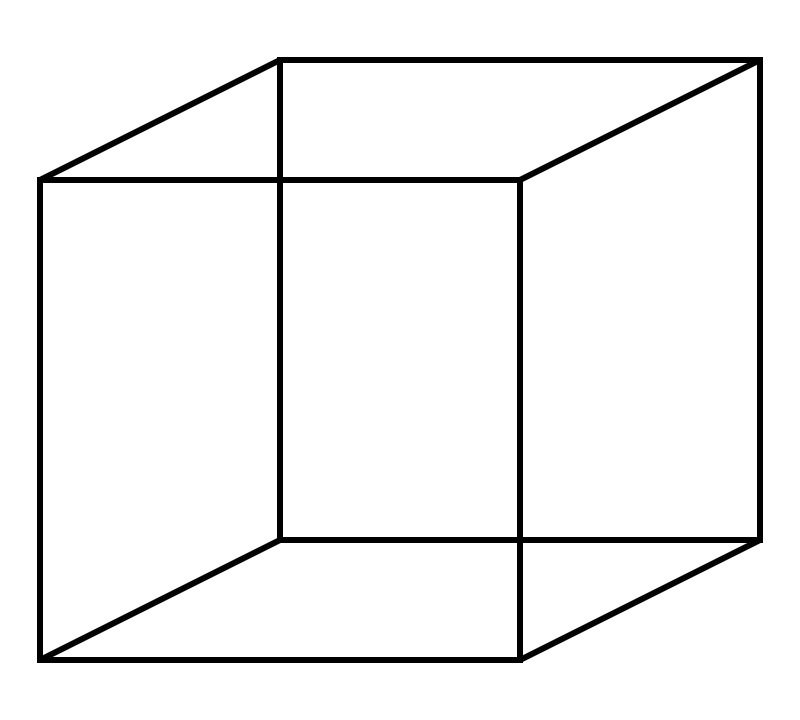
\includegraphics[width=\textwidth,height=0.6\textheight]{../images/necker.png}

}

\caption{The necker cube 'illusion}

\end{figure}
\end{frame}

\begin{frame}{Voluntary Control}
\protect\hypertarget{voluntary-control-1}{}
\begin{itemize}[<+->]
\tightlist
\item
  Stage 3 doesn't seem to be voluntary; you can't just decide that this
  experience is good evidence that it will snow tonight.
\item
  Stage 4 does seem voluntary; actions are paradigmatically voluntary
  (in normal circumstances)
\end{itemize}
\end{frame}

\begin{frame}{Voluntary Control}
\protect\hypertarget{voluntary-control-2}{}
\begin{itemize}[<+->]
\tightlist
\item
  We'll want to come back to this point; you might think given the focus
  of epistemologists on stage 3, it should be \textbf{more} voluntary
  than the others.
\end{itemize}
\end{frame}

\begin{frame}{Skill}
\protect\hypertarget{skill}{}
Seems pretty clear that 1, 3 and 4 can show skill.

\begin{itemize}[<+->]
\tightlist
\item
  Looking in the right places is a skill.
\item
  Drawing the right inferences is a skill.
\item
  Acting sensibily is a skill.
\end{itemize}
\end{frame}

\begin{frame}{Skilled Looking}
\protect\hypertarget{skilled-looking}{}
What's interesting is how much 2 seems to be a skill as well.

\begin{itemize}[<+->]
\tightlist
\item
  An expert musician can \emph{hear} what's wrong with an
  instrument/performance.
\item
  A skilled neo-natal nurse can \emph{see} that a baby is jaundiced.
\end{itemize}
\end{frame}

\begin{frame}{Skill}
\protect\hypertarget{skill-1}{}
There doesn't seem to be any difference between the steps here.
\end{frame}

\begin{frame}{Penetration}
\protect\hypertarget{penetration}{}
For better or worse, the term `cognitive penetration' has become to
standard term for when a part of the mind is sensitive to other beliefs
the person has.

\begin{itemize}[<+->]
\tightlist
\item
  A big question in philosophy and psychology for the last few decades
  has been how much cognitive penetration there is, and should be.
\end{itemize}
\end{frame}

\begin{frame}{Belief}
\protect\hypertarget{belief}{}
Imagine that as leaving this classroom, you have the experience as of
glancing an elephant from the corner of your eye.

\begin{itemize}[<+->]
\tightlist
\item
  You should (and probably would) believe this is some kind of illusion.
\end{itemize}
\end{frame}

\begin{frame}{Belief}
\protect\hypertarget{belief-1}{}
Imagine that as leaving this classroom, you have the experience as of
glancing an elephant from the corner of your eye.

\begin{itemize}[<+->]
\tightlist
\item
  This isn't a zoo, and getting an elephant up those stairs (or worse
  still, into those awful elevators) would be tough.
\end{itemize}
\end{frame}

\begin{frame}{Belief}
\protect\hypertarget{belief-2}{}
What you believe on the basis of an experience is, and should be,
sensitive to what else you believe.

\begin{itemize}[<+->]
\tightlist
\item
  As we sometimes put it, belief formation should be holistic.
\end{itemize}
\end{frame}

\begin{frame}{Experience}
\protect\hypertarget{experience}{}
Big questions:

\begin{enumerate}[<+->]
\tightlist
\item
  How much is experience sensitive to what we antecedently believe?
\item
  How sensitive should it be?
\end{enumerate}
\end{frame}

\begin{frame}{Experience}
\protect\hypertarget{experience-1}{}
One view:

\begin{itemize}[<+->]
\tightlist
\item
  Experience is, and should be, isolated from belief.
\item
  If someone sets up a careful illusion as of an elephant in the
  hallway, you should (and probably would) quickly infer that it is an
  illustion.
\item
  But you should, and probably would, get the illusory experience. You'd
  have the experience of an elephant.
\end{itemize}
\end{frame}

\begin{frame}{Experience}
\protect\hypertarget{experience-2}{}
Of course, things can't be quite this simple.

\begin{itemize}[<+->]
\tightlist
\item
  Skill can change how the world looks. Think again about the musician
  or the nurse.
\item
  But the thought on this view is that belief alone doesn't do that;
  it's a distinct task to acquire this skill.
\end{itemize}
\end{frame}

\begin{frame}{Siegel's Position}
\protect\hypertarget{siegels-position}{}
\begin{enumerate}[<+->]
\tightlist
\item
  Background beliefs can affect experiences themselves, not just what
  conclusions we draw from them.
\item
  While this could be good, if the background beliefs are irrational,
  and especially if they are pernicious, as in the case of racist or
  otherwise prejudiced beliefs, the experiences themselves are
  irrational.
\end{enumerate}
\end{frame}

\begin{frame}{Siegel's Position}
\protect\hypertarget{siegels-position-1}{}
That is, we can ask about the rationality of the irritation
\(\rightarrow\) experience transition, along with other transitions in
the perceptual process.
\end{frame}

\hypertarget{experience-modification-as-a-good}{%
\section{Experience Modification as a
Good}\label{experience-modification-as-a-good}}

\begin{frame}{Helping and Hijacking}
\protect\hypertarget{helping-and-hijacking}{}
The big theme of this chapter is that experience can be
\textbf{hijacked} by bad prior beliefs.

\begin{itemize}[<+->]
\tightlist
\item
  Side note: I'm calling these beliefs, but there is a \emph{big} debate
  about whether prejudices in general are beliefs. Maybe we'll come back
  to that.
\end{itemize}
\end{frame}

\begin{frame}{Helping and Hijacking}
\protect\hypertarget{helping-and-hijacking-1}{}
The big theme of this chapter is that experience can be
\textbf{hijacked} by bad prior beliefs.

\begin{itemize}[<+->]
\tightlist
\item
  Worth spending some time on the case where they are influenced by good
  beliefs.
\item
  What's the best word here? Not hijacked really.
\end{itemize}
\end{frame}

\begin{frame}{Good Cases}
\protect\hypertarget{good-cases}{}
Some of the skilled observing cases I talked about earlier are like
this.

\begin{itemize}[<+->]
\tightlist
\item
  Plausibly linguistic interpretation is like this too.
\end{itemize}
\end{frame}

\begin{frame}{Good Cases}
\protect\hypertarget{good-cases-1}{}
\begin{itemize}[<+->]
\tightlist
\item
  Chess players are better at remembering positions of pieces on a
  board, but that advantage falls away a lot when the positions are not
  real game positions.
\item
  Your experience of these very words is affected by the fact that you
  know that they are words, and what they mean.
\end{itemize}
\end{frame}

\begin{frame}{Good Process, Bad Results}
\protect\hypertarget{good-process-bad-results}{}
There are some amusing cases where these two things interfere.

\begin{itemize}[<+->]
\tightlist
\item
  One of these, that you're probably familiar with, is the Stroop
  effect.
\item
  On the next slide, say (to yourself) as quickly as possible the colors
  that each word is written in.
\end{itemize}
\end{frame}

\begin{frame}
\begin{columns}[T]
\begin{column}{0.25\textwidth}
\Large{ \textcolor{Blue}{Blue} \\ \textcolor{Brown}{Brown}  \\ \textcolor{ForestGreen}{Green} }
\end{column}

\begin{column}{0.25\textwidth}
\Large{  \textcolor{Purple}{Purple}    \\  \textcolor{BrickRed}{Red}    \\     \textcolor{Yellow}{Yellow} }
\end{column}

\begin{column}{0.25\textwidth}
\Large{  \textcolor{Aquamarine}{Teal} \\  \textcolor{Black}{Black} \\  \textcolor{Rhodamine}{Pink} }
\end{column}
\end{columns}
\end{frame}

\begin{frame}
Let's try it again, with some rotations.
\end{frame}

\begin{frame}
\begin{columns}[T]
\begin{column}{0.25\textwidth}
\Large{ \textcolor{Blue}{Red} \\ \textcolor{Brown}{Yellow}  \\ \textcolor{ForestGreen}{Teal} }
\end{column}

\begin{column}{0.25\textwidth}
\Large{  \textcolor{Purple}{Black}    \\  \textcolor{BrickRed}{Pink}    \\     \textcolor{Yellow}{Blue} }
\end{column}

\begin{column}{0.25\textwidth}
\Large{  \textcolor{Aquamarine}{Brown} \\  \textcolor{Black}{Green} \\  \textcolor{Rhodamine}{Purple} }
\end{column}
\end{columns}
\end{frame}

\begin{frame}{Hijacking}
\protect\hypertarget{hijacking}{}
Typically, people who can read English will do worse on this than people
who cannot.

\begin{itemize}[<+->]
\tightlist
\item
  Next week, we'll move on to chapters 2 and 3, and talk about how this
  might affect the rationality of perception.
\end{itemize}
\end{frame}



\end{document}
